\chapter{Framework Valutati}
	Il primo passo necessario nella valutazione di questi framework è stato 
	chiarire bene il fine del loro impiego. Durante la fase di ricerca abbiamo 
	notato una gran confusione nell'attribuire a ciascun framework il tipo di
	applicazione che permetteva di realizzare. Spesso il fatto che 
	l'applicazione venisse eseguita all'interno di una componente nativa veniva 
	pubblicizzato come se il framework fosse in grado di creare una completa 
	applicazione nativa (anziché ibrida); in altri casi 
	veniva confuso il concetto di \crosscomp 
	(\hyperref[sec:nativapp]{vedi~\ref{sec:nativapp}}) con quello di 
	applicazione ibrida; in altri ancora non veniva mostrata la separazione 
	concettuale che vi è tra framework utili per la sola costruzione della 
	logica e dell'interfaccia grafica dell'applicazione e framework che 
	permettono d'incapsulare il contenuto web in una componente nativa creando 
	così un'applicazione ibrida.
	
	Allo scopo di dare ordine per descrivere al meglio le differenze tra i vari 
	framework abbiamo ritenuto opportuno suddividerli a seconda del tipo di 
	applicazioni che sono in grado di produrre.
	
	Abbiamo così classificato Titanium Appcelerator come framework per la 
	realizzazione di applicazioni native; Phonegap/Cordova, Rho Mobile e Sencha 
	Touch come quelli dediti alla creazione di applicazioni ibride; \jqm{},
	\kendomob{} e \phonejs{} utili per implementare complete 
	applicazioni web e per la logica e l'interfaccia grafica di applicazioni 
	ibride.

	\section{Framework per Applicazioni Native}
		
		\subsection{Titanium Appcelerator}
		\label{sec:titanium}
			Titanium è una piattaforma gratis e open source di sviluppo di 
			applicazioni mobili che permette la creazione di applicazioni native
			\crossplat{} per iOS, Android, BlackBerry e Tizen usando il 
			linguaggio \js{}. Usando \js{} e \html{} è anche possibile
			creare semplici applicazioni Web.
			
			Titanium agisce come un ponte tra i sistemi operativi nativi e il 
			codice dell'applicazione. La figura \ref{fig:ti_stack} illustra 
			questa architettura.
			\begin{figure}[h]
				\centering
				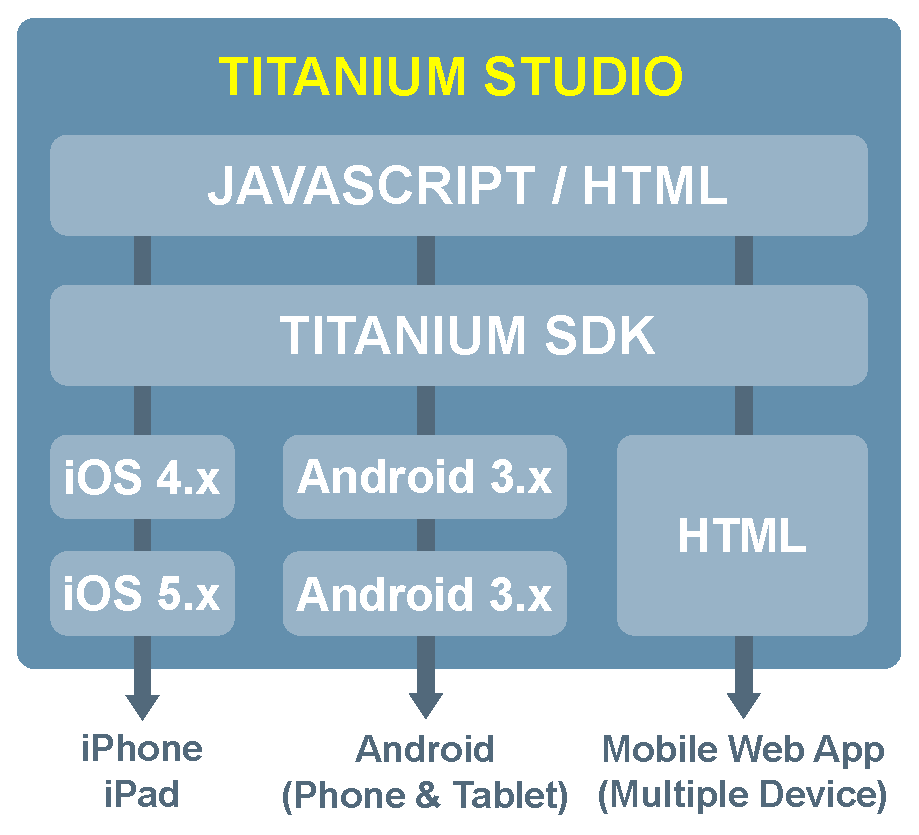
\includegraphics[keepaspectratio=true, width=12cm]{titanium-stack.eps}
				\caption{
					Architettura nello sviluppo di un applicazione \crossplat{} 
					mediante Titanium Studio.
				}
				\label{fig:ti_stack}
			\end{figure}
			In fondo alla pila si trova il sistema 
			operativo di destinazione: Android, iOS o il browser (per quanto 
			riguarda le applicazioni web); sulla cima troviamo il codice 
			dell'applicazione scritta in \js{} e in mezzo trova posto
			Titanium SDK insieme alle proprie APIs. Utilizzando tali interfacce 
			nella propria applicazione è possibile fare azioni come mostrare la 
			fotocamera,	aprire nuove finestre, disegnare pulsanti, ecc. 
			
			Titanium è descritto come un framework \crosscomp{}\citep{Web:peptechlearn.blogspot.it} anche se l'uso che si fa di 
			questo appellativo in questo caso non è del tutto corretto. Come 
			spiega lo stesso amministratore delegato di Appcelerator Inc., Jeff 
			Haynie, in un intervento online su 
			\mbox{stackoverflow.com}\footnote{In quell'occasione era stato 
			chiesto proprio come Titanium potesse funzionare riguardo alla 
			creazione del codice nativo.\\L'intera discussione è consultabile 
			all'indirizzo 
			\url{http://stackoverflow.com/questions/2444001/how-does-appcelerator-titanium-mobile-work}}
			il modo di operare di Titanium è il seguente:
			\begin{quotation}
				Titanium takes your \js{} code, analyzes and preprocesses 
				it and then pre-compiles it into a set of symbols that are 
				resolved based on your applications uses of Titanium APIs. From 
				this symbol hierarchy we can build a symbol dependency matrix 
				that maps to the underlying Titanium library symbols to 
				understand which APIs (and related dependencies, frameworks, 
				etc) specifically your app needs. I'm using the word symbol in a 
				semi-generic way since it's a little different based on the 
				language. In iPhone, the symbol maps to a true C symbol that 
				ultimately maps to a compiled .o file that has been compiled for 
				ARM/i386 architectures. For Java, well, it's more or less a 
				.class file, etc. Once the front end can understand your 
				dependency matrix, we then invoke the SDK compiler (i.e. GCC for 
				iPhone, Java for Android) to then compile your application into 
				the final native binary.
				
				So, a simple way to think about it is that your JS code is 
				compiled almost one to one into the representative symbols in 
				nativeland. There's still an interpreter running in interpreted 
				mode otherwise things like dynamic code wouldn't work. However, 
				its much faster, much more compact and it's about as close to 
				pure native mapping as you can get. [\ldots]
			\end{quotation}
			Ciò significa che il sistema fa tutto il possibile per creare codice 
			nativo che rappresenti uno a uno quello che si è descritto in 
			\js{} ma parte del nostro sorgente dovrà ancora essere 
			interpretato a tempo di esecuzione. L'interprete \js{} viene 
			inserito nel pacchetto in fase di compilazione e, a seconda della 
			piattaforma di destinazione, sarà inserito 
			\js{}Core\footnote{Maggiori dettagli e informazioni si possono 
			trovare online all'indirizzo\\ \url{http://webkit.org/projects/javascript/}} 
			per iOS o Rhino\footnote{Maggiori dettagli e informazioni si possono trovare 
			online all'indirizzo\\ \url{https://developer.mozilla.org/it/docs/Rhino}} 
			per Android e BlackBerry\citep{Web:KevinPost}.
			
			Visto che il codice \js{} viene ancora in parte interpretato, 
			\crosscomp{} non è del tutto appropriato in quanto con tale 
			aggettivo ci si riferisce ad una tecnica che permette, a partire da 
			un certo sistema, di creare codice eseguibile per un secondo sistema 
			avente caratteristiche e proprietà differenti da quello di 
			partenza\citep{Web:Wiki.cross-compiling}.
			
			In ogni caso possiamo pensare di utilizzare il termine 
			\crosscomp{} per indicare che Titanium, al termine del processo di 
			compilazione, produce un pacchetto che per la 
			maggior parte contiene codice nativo e specifico per una data 
			piattaforma. Questa è una differenza sostanziale rispetto a quello 
			che avviene nella compilazione di un'applicazione ibrida, dove nel 
			pacchetto risultante è solo il codice della web view ad essere 
			realizzato in codice nativo, mentre il codice sorgente web 
			(\js{}, \html{} e \css{}) rimane intatto e viene poi interpretato 
			completamente dal motore del browser a tempo di esecuzione.
			
			Titanium richiede che sulla macchina usata per lo sviluppo vengano 
			installati e configurati gli SDK nativi per le piattaforme di 
			destinazione. In particolare per le applicazioni Android bisogna 
			installare l'Android SDK, mentre serve Xcode per le applicazioni 
			iOS. Questo perchè dopo la prima fase di elaborazione dei sorgenti 
			fatta dallo SDK di Titanium (descritta nell'intervento succitato) 
			serve usare l'SDK nativo per creare il pacchetto finale da 
			installare sul dispositivo.
			
			\clearpage
			\noindent Detto questo passiamo ad elencare cosa Titanium offre da 
			una visione più ad alto livello\citep[Cap.2 - Titanium 
			Mobile Overview]{Book:Ti}:
			\begin{itemize}
				\item Strumenti dello SDK Titanium
				\item APIs Mobile
				\item Titanium Studio
				\item Moduli
				\item Servizi cloud di Appcelerator
			\end{itemize}
	
			\paragraph{Strumenti dello SDK Titanium}
				Come strumenti per compilare l'applicazione in un pacchetto 
				installabile contenente codice nativo, Titanium SDK utilizza un 
				insieme di script Python e altri strumenti di supporto che 
				lavoreranno insieme a quelli forniti dagli SDK per lo sviluppo 
				nativo\footnote{Da qui la necessità di lavorare in un ambiente 
				configurato con gli SDK nativi delle piattaforme per le quali si 
				desidera realizzare l'applicazione}. Tutto questo è trasparente 
				agli occhi di uno sviluppatore che può così concentrarsi solo 
				nella realizzazione della propria applicazione.
				
			\paragraph{APIs Mobili}
				Titanium fornisce un ricco insieme di API \js{} che danno 
				accesso a centinaia tra componenti native per l'interfaccia 
				utente e componenti non visuali. Queste API sono suddivise in 
				vari insiemi come Titanium.UI (per quanto riguarda l'interfaccia 
				utente) o Titanium.Network (per quanto riguarda il networking).
				 
			\paragraph{Titanium Studio}
				Appcelerator mette anche a disposizione un proprio IDE gratuito 
				per rendere più agevole lo sviluppo. Titanium Studio, appunto, è 
				un ambiente di sviluppo integrato derivato da Eclipse, uno degli 
				IDE open-source più utilizzati. Con Titanium Studio è possibile 
				scrivere, fare testing e debugging delle proprie applicazioni; 
				inoltre sono presenti anche vari templates e applicazioni di 
				esempio per rendere più semplice incominciare a creare 
				applicazioni con Titanium SDK. Titanium Studio è stato 
				pensato per essere l'unico software di cui si ha bisogno (oltre 
				agli SDK nativi delle diverse piattaforme) per incominciare a 
				sviluppare con Titanium SDK; per questo motivo dal suo interno 
				si ha la possibilità di installare e configurare l'SDK (al primo 
				avvio) e successivamente eseguire aggiornamenti. In più è
				integrata la funzionalità che permette di scaricare nuovi moduli 
				per	estendere l'insimeme delle APIs.
				
				L'uso di questo strumento non è obbligatorio, Titanium SDK 
				ha una propria interfaccia a linea di comando che permette di 
				gestire ogni aspetto dello sviluppo: inizializzare un 
				nuovo progetto, compilarlo, eseguirlo e permette anche di 
				installare nuovi aggiornamenti dello SDK nonché di configurarlo.
				Ovviamente se si rinuncia a Titanium Studio non è garantito che 
				si riescano a trovare i medesimi tool per il debugging in altri 
				IDE che si possono trovare in quello fornito da Appcelerator.
				
			\paragraph{Moduli}
				Titanium è composto da una serie di moduli che estendono alcune 
				funzioni principali delle API. Se si controlla la documentazione 
				relativa si può trovare una lista di moduli base che estendono 
				il nucleo del sistema e, inoltre, Appcelerator pubblica 
				campioni di moduli gratuiti sul proprio repository git su 
				\mbox{github.com}\footnote{Il repository ufficiale di tutti i 
				moduli pubblicati è	raggiungibile all'indirizzo\\
				\url{https://github.com/appcelerator/titanium_modules}}. 
				Ovviamente ogni sviluppatore è libero di creare e distribuire 
				gratuitamente o vendere i proprio moduli attraverso il 
				Marketplace\footnote{Appcelerator Marketplace\\
				\url{https://marketplace.appcelerator.com/}} 
				di Appcelerator. Titanium SDK supporta l'impiego dei moduli 
				anche nello sviluppo delle applicazioni web, in questo caso la 
				loro realizzazione consiste nello scrivere un puro modulo 
				\js{} e non qualcosa scritto in Java o Objective-C.
			
			\clearpage
			\paragraph{Servizi cloud di Appcelerator}
				Appcelerator fornisce svariati servizi ACS (Appcelerator Cloud 
				Services) che sono inclusi nella lista delle varie componenti 
				fruibili attraverso le API. Alcune delle funzionalità offerte da 
				questi servizi sono:
				\begin{itemize}
					\item Invio di notifiche push
					\item Gestione dell'utente
					\item Salvataggio e manipolazione di foto
					\item Integrazioni con i social network
					\item Memorizzazione di file
					\item Chat
					\item Memorizzazione di dati in formato chiave-valore
				\end{itemize}
				Per poter usufruire dei servizi ACS nella propria applicazione, 
				otre che ad utilizzare le relative API fornite è necessario 
				registrare la propria app online sul sistema di gestione dei 
				servizi ACS di Appcelerator.
			
			\subsubsection{Titanium SDK e il paradigma MVC}
				Appcelerator fornisce il framework Alloy che consente agli 
				sfiluppatori di strutturare le loro applicazioni secondo 
				paradigma MVC (Model-View-Controller)\footnote{Per approfondire 
				si può consultare l'indirizzo\\
				\url{http://en.wikipedia.org/wiki/Model-view-controller}}. Con 
				questo framework l'interfaccia viene costruita combinando file 
				sorgenti scritti con i linguaggi XML e \css{} mentre il codice che 
				riguarda la logica dell'applicazione è ancora \js{}. 
				L'uso di Alloy necessita di un passaggio in più durante il 
				processo di compilazione: i vari file sorgenti di 
				un'applicazione Alloy vengono ``pre-compilati'' per generare 
				tradizionali sorgenti \js{} di un'applicazione Titanium.
				
				In fase di inzializzazione di un nuovo progetto, Titanium Studio 
				permette di impiegare o meno Alloy nello sviluppare 
				l'applicazione; in ogni caso il processo di compilazione è, come 
				già detto, completamente gestito da Titanium SDK e rimane 
				invisibile allo	sviluppatore.
			
	\section{Framework per Applicazioni Web}	
	\label{sec:frameworkwebapp}
	
		Come descritto più volte questi framework hanno una duplice funzionalità.
		Ognuno di essi può essere utilizzato indipendentemente per realizzare
		applicazioni web (\hyperref[sec:webapp]{vedi~\ref{sec:webapp}}), oppure 
		può essere combinato ai framework descritti nella 
		sezione\hyperref[sec:frameworkhybrid]{~\ref{sec:frameworkhybrid}} per
		realizzare un'applicazione ibrida più soddisfacente.
		
		\subsection{JQuery Mobile}
		\label{subsec:jQuery}
			\jqm{} è un framework per lo sviluppo di applicazioni mobili
			web	che sono accessibili da tutti i dispositivi: smartphone, tablet
			e computer desktop. Esso è stato costruito sopra i robusti framework
			\jq{} e \jq{} UI, che erano stati sviluppati per potenziare e
			agevolare la creazione dei tradizionali siti web. 
			
			Per usare \jqm{} è sufficiente scaricare dal sito del
			produttore\footnote{\url{http://jquerymobile.com/download/}} il
			pacchetto in formato .zip contenente tutti i file \js{}, \css{} e
			PNG necessari\footnote{Dallo stesso sito c'è la possibilità di
			personalizzare il contenuto del pacchetto .zip in base alle proprie
			preferenze. Ad esempio è possibile alleggerire il pacchetto
			eliminando il supporto per le animazioni di transizione tra le
			pagine}. Una volta ottenuti, questi file vanno inclusi nella pagina
			\html{} che conterrà il codice della struttura dell'applicazione. A
			questo punto è sufficiente scrivere i normali tag \html{} decorati con
			particolari attributi \verb|data-*| per definire i vari componenti
			dell'interfaccia grafica dell'applicazione. Nel esempio \ref{cod:jquery}
			viene mostrata l'implementazione di un'applicazione composta da
			una sola schermata che al suo interno contiene un'intestazione con
			il titolo dell'applicazione e un semplice bottone con un icona a
			forma di ingranaggio.\clearpage
			\begin{lstlisting}[
				label={cod:jquery},
				caption={
					Semplice applicazione jQuery Mobile. Da notare i riferimenti
					aggiunti nell'intestazione del documento HTML necessari per
					l'uso del framework.
				}
			]
	<!DOCTYPE html>
	<html>
		<head>
			<meta name="viewport" content="initial-scale=1, maximum-scale=1">
			<link
				rel="stylesheet"
				href="jquery.mobile-1.4.2.min.css" />
			<script src="jquery-1.9.1.min.js"></script>
			<script src="jquery.mobile-1.4.2.min.js"></script>
		</head>
		<body>
			<div data-role="page">
				<div data-role="header">
					<h1>jQuery Mob. App</h1>
				</div>
				<a data-icon="gear" class="ui-btn">Options</a>
			</div>
		</body>
	</html>
			\end{lstlisting}
			\jqm{} in fase di inizializzazione seleziona gli elementi in
			base ai loro attributi \verb|data-*| e li potenzia inserendo dei markup
			aggiuntivi aggiungendo nuove classi \css{} e applicando gestori per gli
			eventi.	Questo permette allo sviluppatore di scrivere velocemente
			una pagina con una certa base semantica, sarà poi \jqm{} a
			dare all'applicazione una più complessa interfaccia utente.	Se
			l'applicazione è composta da più schermate \jqm{} fornisce 
			il concetto di pagina per poter modellare questi elementi e
			implementa anche un sistema di navigazione \ajax{} (Asynchronous
			\js{} and XML) per supportare un ricco insieme di animazioni
			nella transizione tra le pagine. Per definire una pagina è
			sufficiente racchiuderne il contenuto in un tag \verb|<div>| con
			l'attributo personalizzato \verb|data-role="page"|.	In uno stesso
			file \html{} possono essere inserite più pagine ma questo non è
			obbligatorio; è possibile usare file \html{} specifici per ogni pagina.
			Quando un utente che sta visualizzando una pagina naviga verso
			un'altra viene generato un evento catturato automaticamente dal
			sistema di navigazione \ajax{} che esegue una richiesta di caricamento
			per la nuova pagina. Se la pagina di destinazione è stata definita
			nello stesso file dove è presente la pagina di partenza si parla di
			navigazione interna, altrimenti si parla di navigazione esterna. Nel
			primo caso essendo già stato caricato il file \html{} entrambe le
			pagine sono presenti nel DOM\footnote{Document Object Model: è il
			modello a oggetti \js{} generato dal browser che rappresenta la
			struttura dell'attuale documento \html{} caricato.} e si avrà una
			veloce transizione animata dagli effetti forniti dal framework;
			nel caso di navigazione esterna si dovrà attendere il caricamento
			del nuovo documento, durante il quale \jqm{} cerca gli
			elementi \html{} con l'attributo \verb|data-role="page"|, crea il
			relativo modello a oggetti e lo inserisce nell'attuale DOM.	In
			entrambi i tipi di navigazione il DOM viene aggiornato con i
			contenuti relativi alla pagina da mostrare e non viene mai
			reinizializzato completamente. Questo comporta navigazioni più
			gradevoli alla vista dell'utente e il sistema di caricamento
			asincrono permette di visualizzare animazioni di caricamento in
			sovrapposizione alla pagina che si stà lasciando fino all'effettiva
			navigazione nella nuova pagina.
			
			\jqm{} mette a disposizione dello sviluppatore numerosi
			widgets (come bottoni, liste scorrevoli, switch, ecc...) per
			comporre l'interfaccia grafica. L'aspetto dell'applicazione può
			essere personalizzato utilizzando molti temi già forniti dal
			produttore; online è presente anche un tool per crearne di nuovi
			\footnote{ThemeRoller è reperibile all'indirizzo
			\url{http://themeroller.jquerymobile.com/}} ma non è fornita la
			funzionalità automatica di adattare l'aspetto a seconda della
			piattaforma sulla quale si sta eseguendo l'applicazione (vedi fig.
			\ref{fig:jquery}).
			
			Il framework consente di essere esteso tramite l'aggiunta di nuovi
			plug-in e widgets personalizzati. Nuovi plug-in permettono di
			estendere le funzionalità del sistema mentre nuovi widgets
			consentono di arricchire l'interfaccia utente.
			\begin{figure}[h]
				\centering
				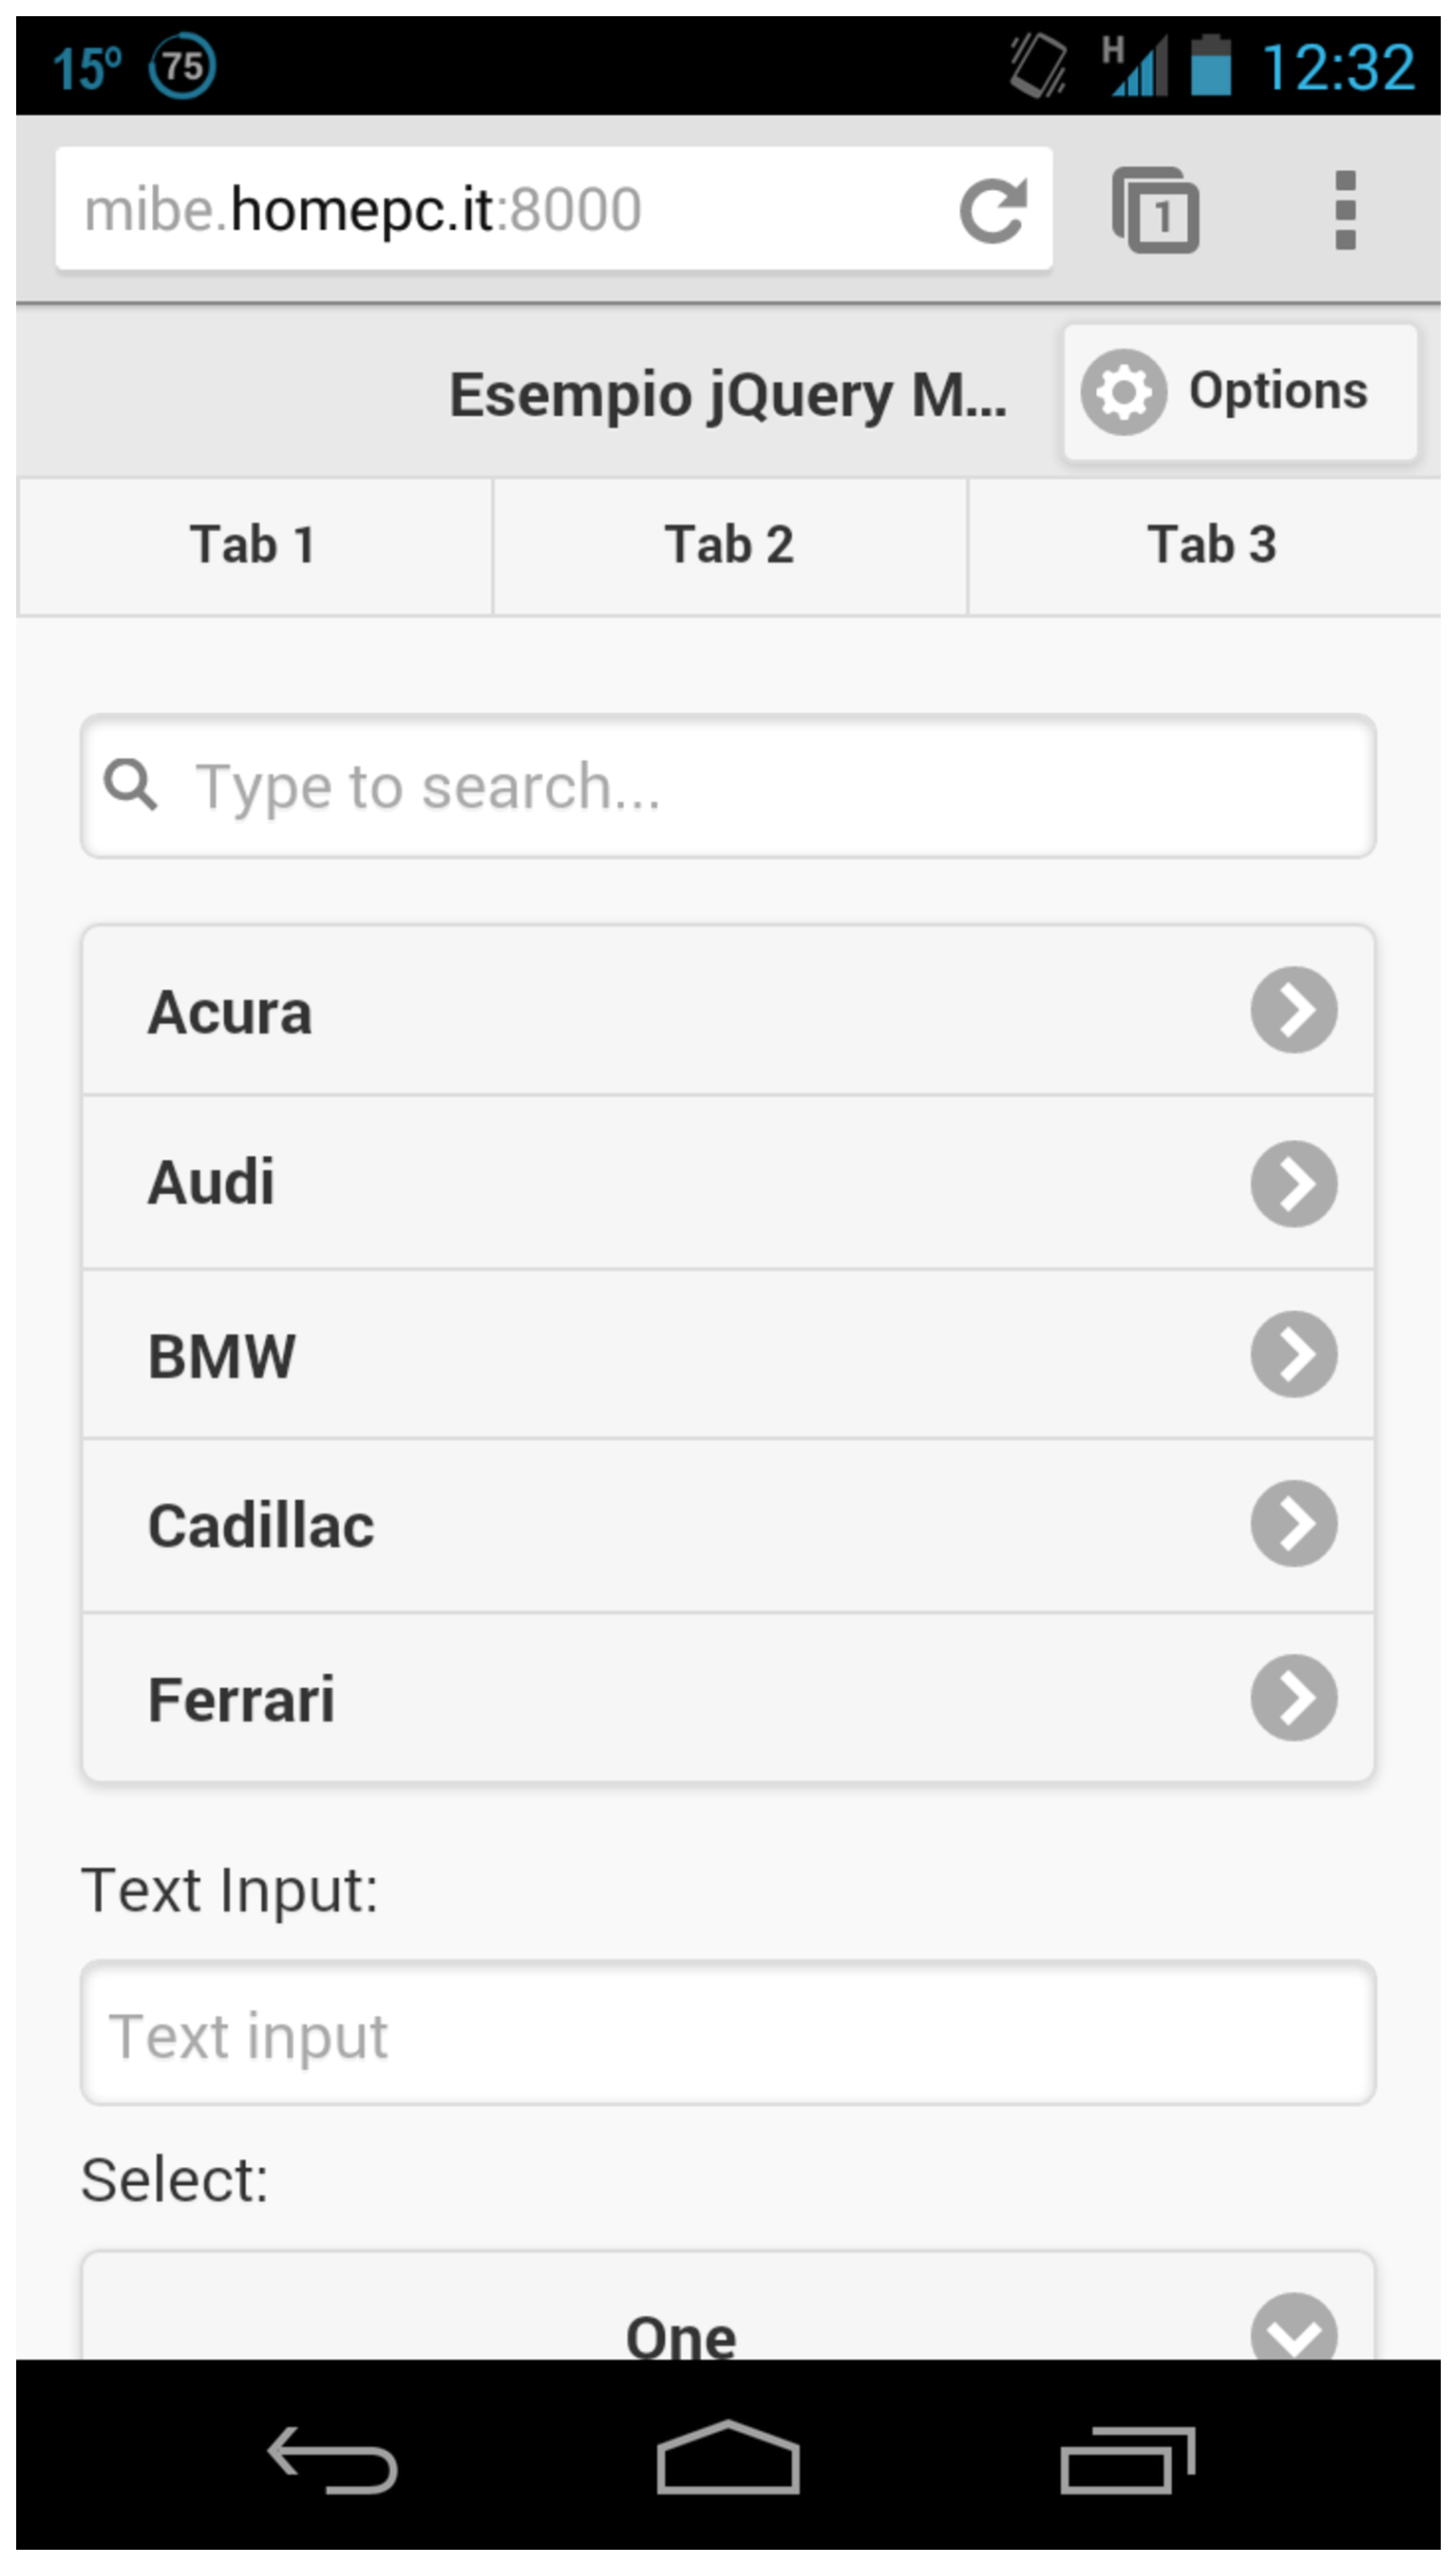
\includegraphics[keepaspectratio=true, width=0.32\textwidth]{jQuery-and}
				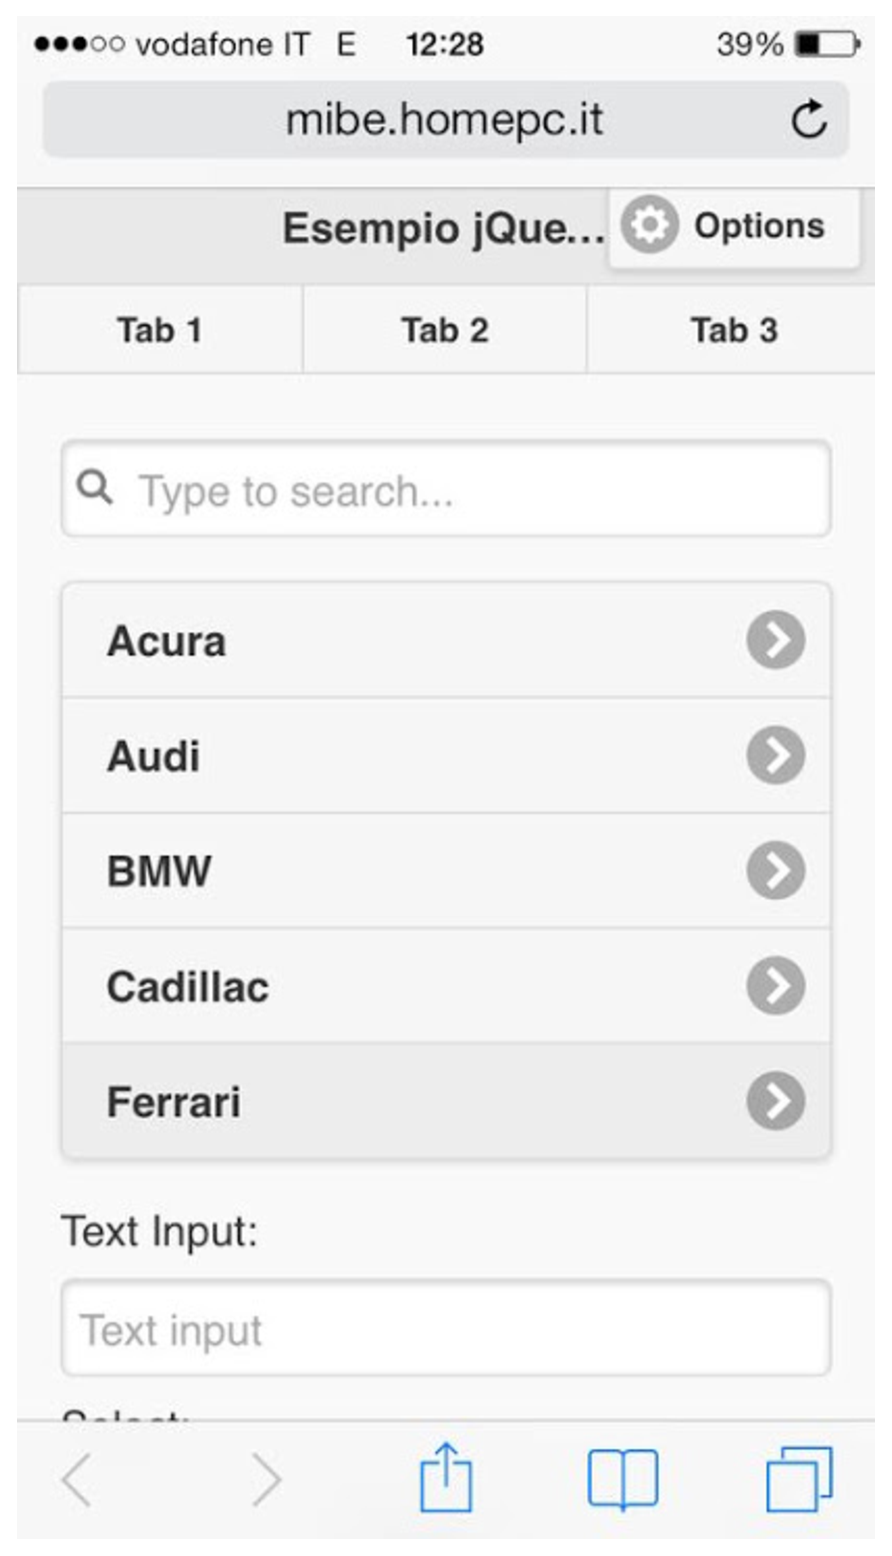
\includegraphics[keepaspectratio=true, width=0.32\textwidth]{jQuery-ios}
				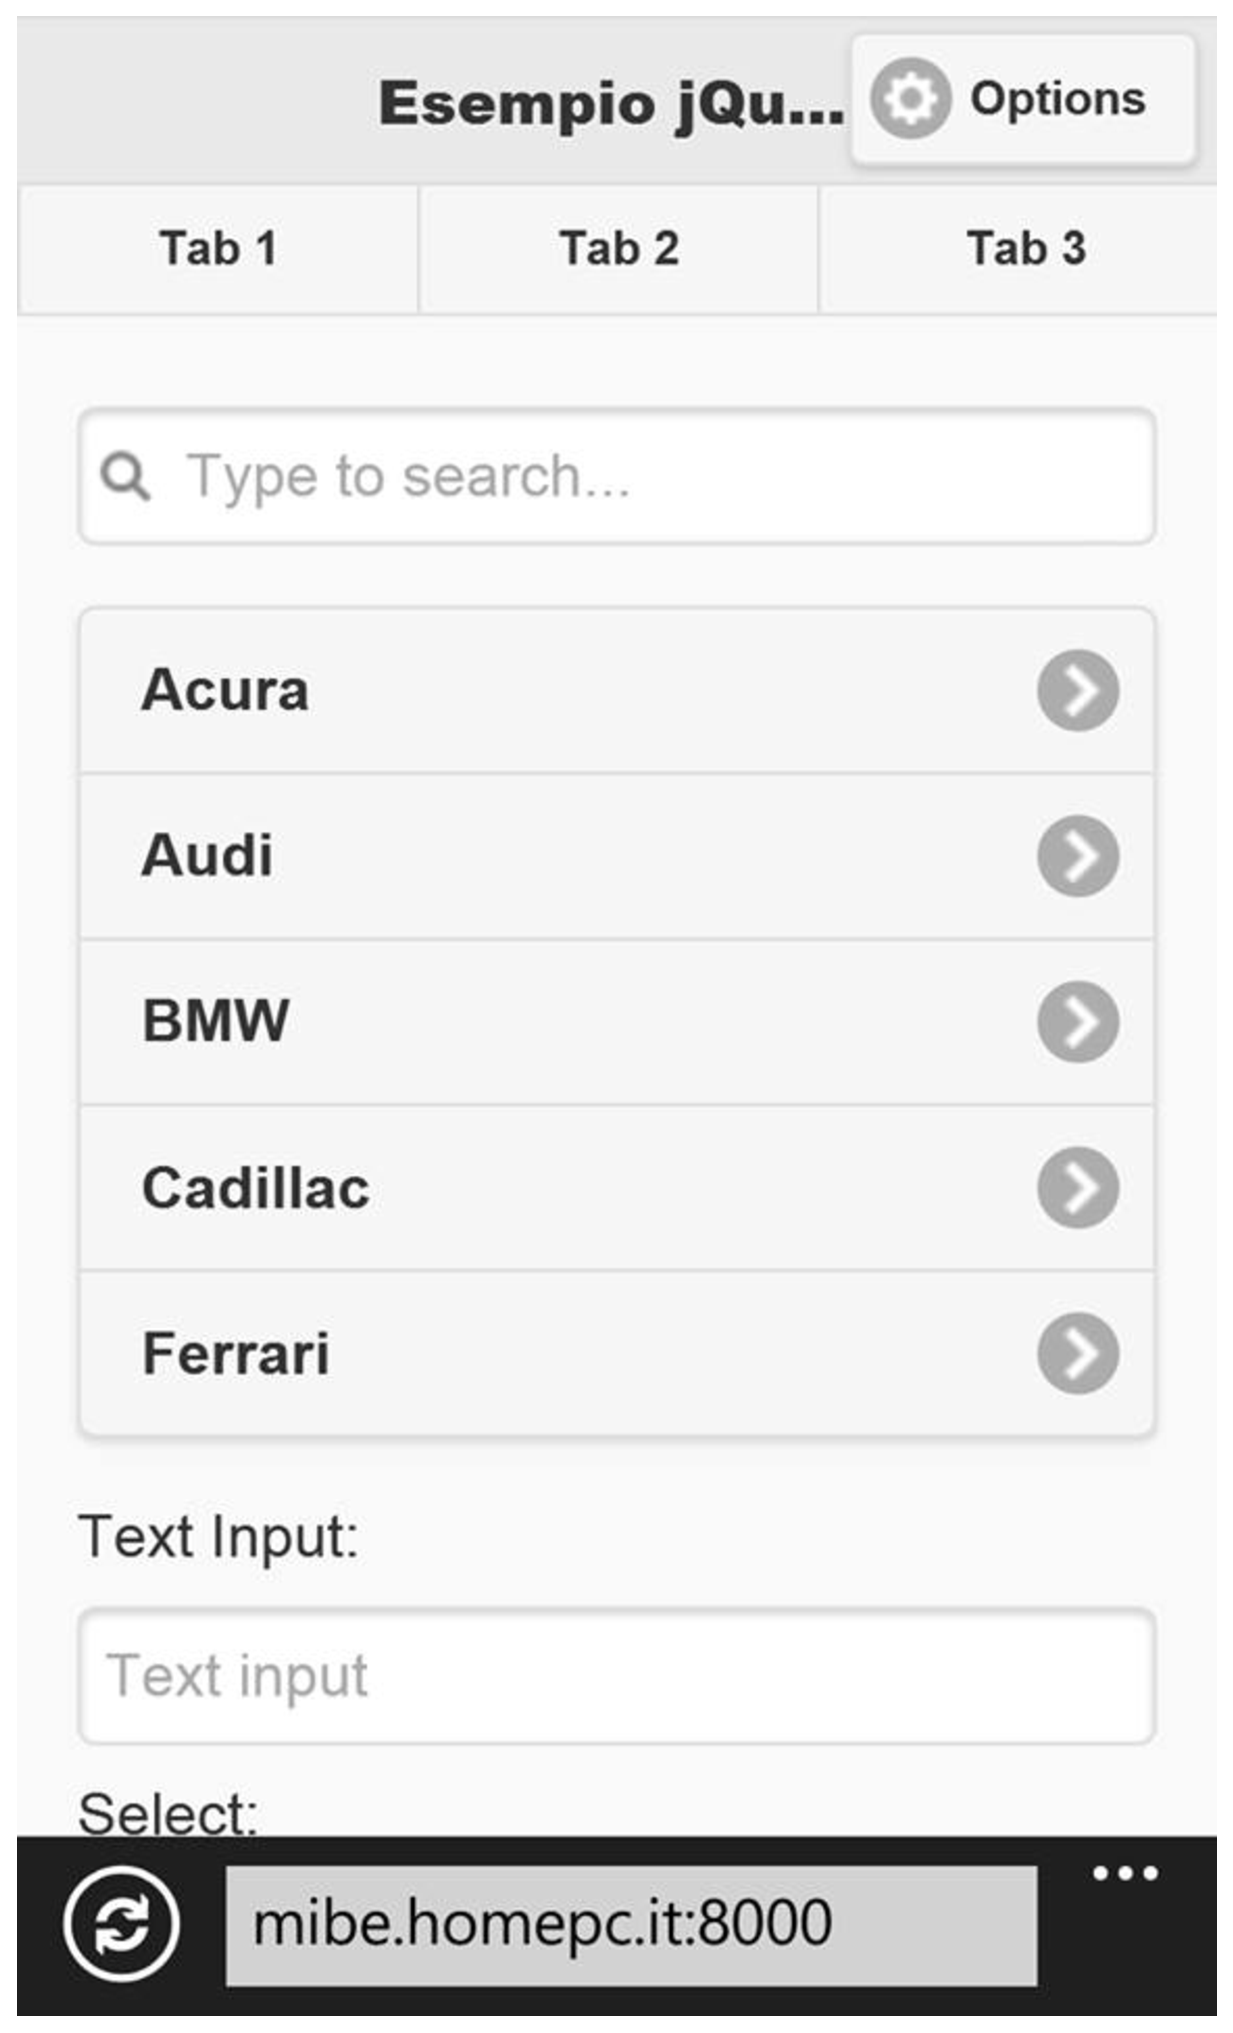
\includegraphics[keepaspectratio=true, width=0.32\textwidth]{jQuery-wp8}
				\caption{
					Un esempio di applicazione web realizzata con \jqm{}.
					Da sinistra a destra l'anteprima su piattaforma Android, iOS
					e WindowsPhone8.
				}
				\label{fig:jquery}
			\end{figure}
	
		\subsection{KendoUI Mobile}
		\label{subsec:kendo}
			\kendomob{} è un framework mobile completo che adatta
			automaticamente	l'aspetto dell'applicazione alla piattaforma sulla
			quale è eseguita. Consiste di estensioni fondamentali per un
			framework mobile come layouts, views, animazioni di transizione,
			e fornisce un ricco insieme di widgets per la costruzione
			dell'interfaccia grafica tra cui bottoni, liste, aree di input di
			testo e altro. Non è però solo per queste caratteristiche che viene
			definito un framework completo, infatti \kendomob{} offre anche
			un utile componente per la gestione di sorgenti data, strumenti di
			validazione degli input, API per la globalizzazione e un framework
			MVVM (Model View ViewModel). Come \jqm{}, \kendomob{} è
			basato sulla libreria \js{} \jq{}.
			
			\kendomob{} in versione di prova è scaricabile dal sito 
			\url{http://www.telerik.com/download/kendo-ui-mobile}, quello che si 
			ottiene è un pacchetto zip contenente tutti i file \js{} e \css{} 
			necessari. La versione di prova	può essere usata per apprendere
			l'uso del framework ma non può essere usata per scopi commerciali 
			quindi, a differenza di \jqm{}, è necessario	mettere in conto
			la spesa di acquisto della licenza se si intende commercializzare
			l'applicazione.	I file \js{} e \css{} scaricati devono essere
			inseriti nel file \html{} che costituisce l'applicazione esattamente
			come è stato descritto per \jqm{}\footnote{Informazioni
			aggiuntive per iniziare a lavorare con \kendomob{} si possono
			trovare nel sito \url{http://docs.telerik.com/kendo-ui/getting-started/introduction}},
			inoltre, è necessario aggiungere uno script di inizializzazione che
			istruisce \kendomob{} su quale parte della pagina \html{} contiene il
			codice che implementa l'applicazione come mostrato nel frammento di
			codice \ref{cod:kendoinit}.
			\begin{lstlisting}[
				label={cod:kendoinit},
				caption={
					Esempio di inizializzazione di un'applicazione KendoUI Mobile
				}
			]
	<!DOCTYPE html>
	<html>
		<head>
			<link href="kendo.mobile.all.min.css" rel="stylesheet" />
			<script src="jquery.min.js"></script>
			<script src="kendo.mobile.min.js"></script>
		</head>
		<body>
			<div data-role="view" data-title="Home"> ... </div>
			<div data-role="view" data-title="Opzioni"> ... </div>
			...
			<script>
				// Inizializza la nuova applicazione KendoUI Mobile
				var app = new kendo.mobile.Application(
					$(document.body)
				);
			</script>
		</body>
	</html>
			\end{lstlisting} 
			Anche \kendomob{} sfrutta gli attributi \verb|data-*| per
			caratterizzare i vari tag \html{} dando loro un particolare aspetto
			grafico relativo al widget che si vuole definire; la stessa
			operazione può essere fatta direttamente da codice \js{}: nel
			framework sono presenti le varie API per poter inizializzare ogni
			widget su un particolare elemento \html{}. Per esempio il frammento di
			codice \ref{cod:htmlbutton} mostra come definire direttamente in
			\html{} un pulsante \kendomob{} mentre nel listato \ref{cod:jsbutton}
			viene definito lo stesso widget ma tramite uno script \js{} che
			può essere anche inserito in un file separato.
			\begin{lstlisting}[
				label={cod:htmlbutton},
				caption={
					Definizione di un bottone KendoUI Mobile in HTML tramite
					attributo {\texttt{data-*}}.
				}
			]
	...
	<div id="foo" data-role="view">
		...
		<a data-role="button">Click Me</a>
	</div>
			\end{lstlisting}
			\begin{lstlisting}[
				label={cod:jsbutton},
				caption={
					Definizione di un bottone KendoUI Mobile in JavaScript
					tramite l'uso delle apposite API.
				}
			]
	...
	<div id="foo" data-role="view">
		...
		<a id="btnClickMe">Click Me</a>
	</div>
	<script>
		$("#btnClickMe").kendoMobileButton();
	</script>
			\end{lstlisting}
			
			Il punto di forza di \kendomob{} è la possibilità di creare
			applicazioni con aspetto nativo. Scrivendo codice una sola volta
			sarà infatti il framework, all'avvio dell'applicazione, ad occuparsi
			di identificare la piattaforma e a applicare il tema corretto. A
			prescindere da questa funzionalità è comunque possibile forzare
			l'utilizzo di uno stesso tema su piattaforme diverse. Attualmente
			\kendomob{} fornisce temi di aspetto nativo per le piattaforme
			Android, iOS, BlackBerry e Windows Phone 8 come mostrato in
			figura~\ref{fig:kendoui} ma, se si ha la necessità, è disponibile
			uno strumento online per la realizzazione dei propri temi
			personalizzati.
			\begin{figure}[h]
				\centering
				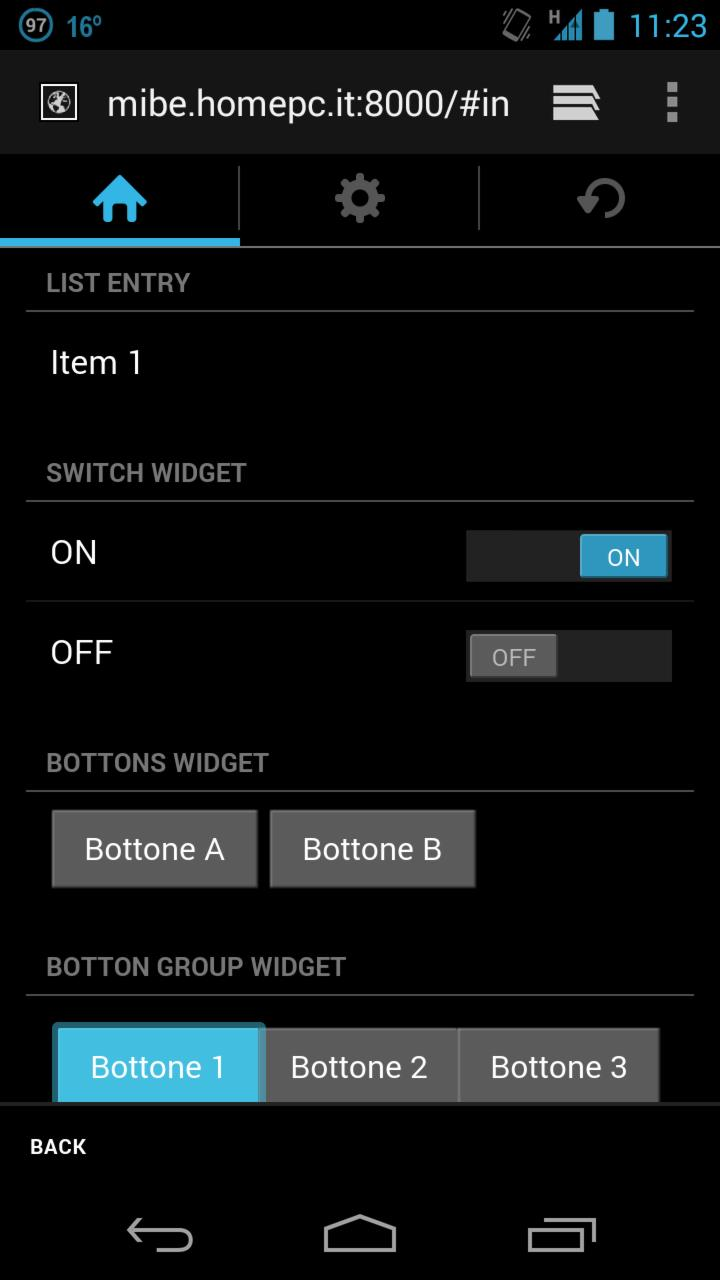
\includegraphics[keepaspectratio=true, width=0.32\textwidth]{kendoui-and}
				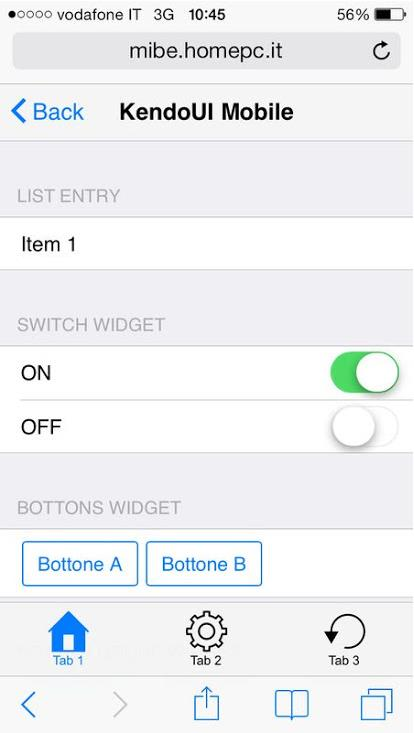
\includegraphics[keepaspectratio=true, width=0.32\textwidth]{kendoui-ios}
				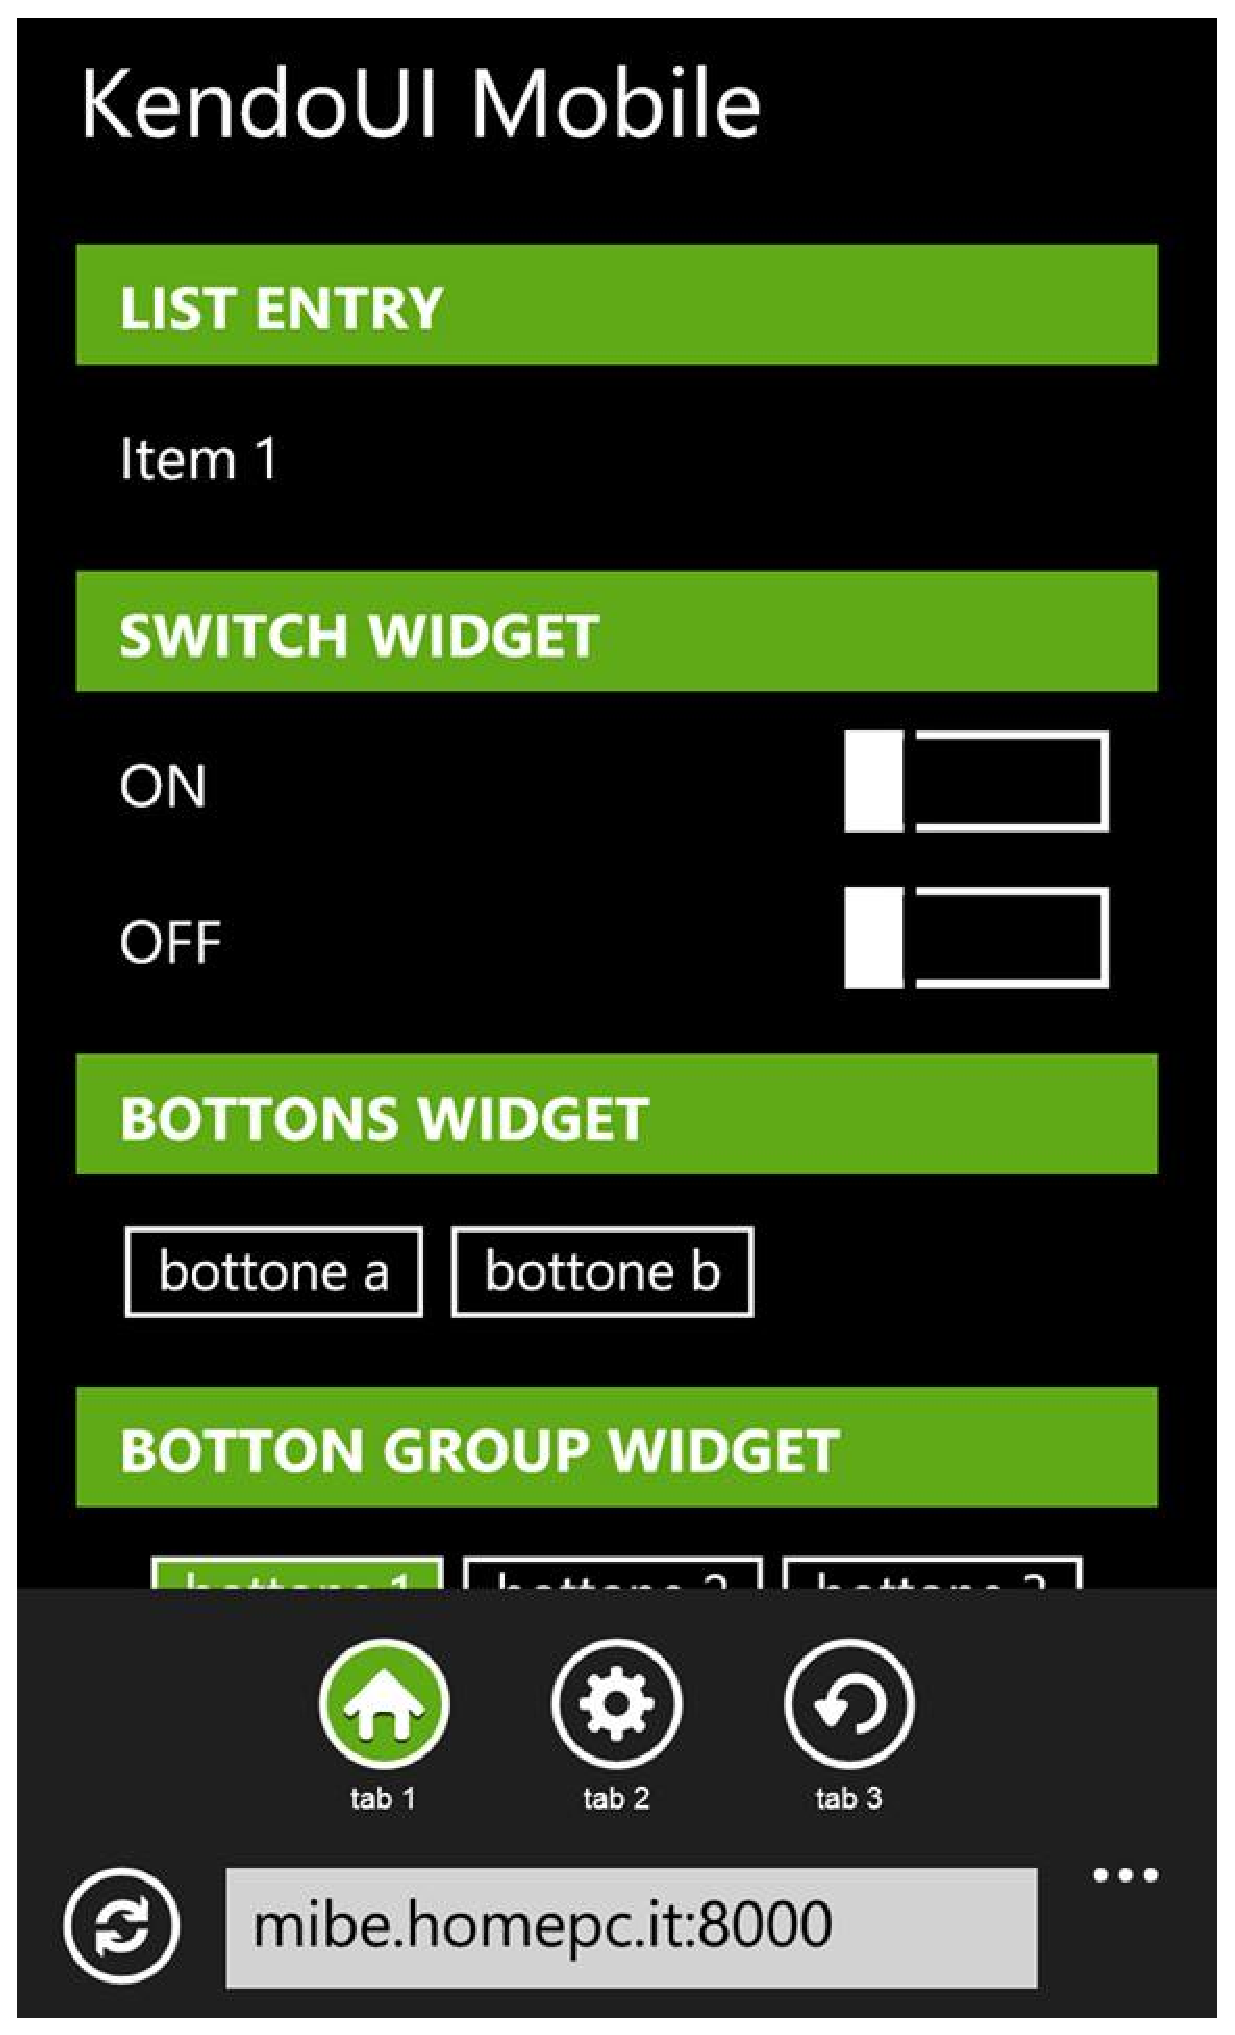
\includegraphics[keepaspectratio=true, width=0.32\textwidth]{kendoui-wp8}
				\caption{
					Un esempio di applicazione web realizzata con \kendomob{}.
					Da sinistra a destra l'anteprima su piattaforma Android, iOS
					e WindowsPhone8.
				}
				\label{fig:kendoui}
			\end{figure}
			ThemeBuilder\footnote{Disponibile online sul sito web del produttore
			all'indirizzo \url{http://demos.telerik.com/kendo-ui/themebuilder/mobile.html}},
			con una semplice interfaccia grafica, consente di modificare colori e
			sfondi delle componenti grafiche dell'applicazione mostrando
			un'anteprima per ogni piattaforma supportata; una volta ottenuto il
			risultato desiderato è possibile esportare il tema in un file \css{} da
			utilizzare poi nella nostra app.
			
			Come precedentemente detto \kendomob{} non offre solo elementi
			di personalizzazione per l'interfaccia grafica. Il componente
			\mbox{DataSource} (KendoUI \mbox{DataSource}) è un'astrazione per la gestione e
			l'impiego di dati locali (array di oggetti \js{}) o remoti
			(XML, JSON, JSONP).	Esso supporta completamente il CRUD (Create,
			Read, Update, Destroy) cioè fornisce le funzioni per creare,
			leggere, aggiornare e distruggere dati e consente sia alla parte
			locale che alla parte server di ordinare, impaginare, filtrare e
			raggruppare questi dati. Molti widgets di \kendomob{} supportano
			il data binding, cioè l'associazione dei dati agli elementi grafici;
			grazie a questo	è possibile ad esempio mostrare in una lista i dati
			letti da un	server o caricati localmente specificando non molto di
			più del formato con	cui questi sono strutturati.

			Come detto poco fa \kendomob{} fornisce un framework per lo
			sviluppo seguendo il paradigma MVVM; per provare a spiegare in cosa
			consiste tale modello ci serviamo di un esempio. Tipicamente in un
			qualsiasi genere di programma o applicazione è cosa comune dover
			manipolare certe entità; un'app che gestisce domande di laurea dovrà
			ragionevolmente trattare studenti, dove uno studente avrà 
			particolari caratteristiche come nome, cognome e numero di matricola.
			Questo avrà due rappresentazioni: una in memoria mediante strutture
			dati opportune e un'altra grafica dove i dati dello studente saranno
			mostrati all'utente attraverso elementi grafici. L'utente può
			inoltre compiere determinate azioni su queste entità attraverso
			elementi grafici (es. sottoporre la domanda di laurea attraverso
			il tocco di un apposito tasto). Il paradigma Mo\-del-\-View-\-View\-Mo\-del 
			formalizza le suddette rappresentazioni rispettivamente come Model e 
			View, inoltre introduce il ViewModel, un terzo elemento che le mette 
			in relazione, consentendo che le azioni e le modifiche fatte da
			parte dell'utente sulla View si ripercuotano sul relativo Model e
			viceversa. Impostare un'applicazione individuando queste parti
			porta alla scrittura di un codice più strutturato, più manutenibile
			nonché più leggibile.
			
			\kendomob{} fornisce un modo per internazionalizzare le pagine che 
			compongono l'applicazione. Attraverso un particolare metodo offerto
			dalle API è possibile selezionare un particolare paese in modo da
			adottarne il formato di rappresentazione dei numeri, nomi dei mesi,  
			di data e ora in maniera conforme agli standard locali.
	
			\html 5 ha introdotto gli attributi di validazione, questi particolari 
			attributi hanno la capacità di forzare il browser ad avvisare
			l'utente che un certo elemento di input contenuto in un form debba
			essere compilato obbligatoriamente.	KendoUI Validator offre un modo
			facile per gestire la validazione per gli elementi input di un form
			permettendo di personalizzare la gestione della validazione, ad
			esempio, accettando in input solo stringhe contenenti certe parole o
			numeri compresi in un dato intervallo.
			
			Come in \jqm{} è possibile realizzare un'intera applicazione
			composta da più schermate in una singola pagina \html{} attraverso l'uso
			del widgets view. Avendo la completa applicazione all'interno di un
			unico file si hanno ovvi vantaggi nella navigazione tra le sue schermate
			come già descritto per \jqm{}
			\hyperref[subsec:jQuery]{(vedi~\ref{subsec:jQuery})}.
			Per accelerare ulteriormente il caricamento delle views, se queste
			presentano la medesima struttura (per esempio sono composte da una
			intestazione contente una barra di navigazione e da un corpo),
			questa può essere definita in un particolare oggetto chiamato layout
			condiviso tra più views.
			
		\subsection{PhoneJS}
			PhoneJS è un framework per realizzare applicazioni mobili 
			single page application (SPA), che promette di fornire: un'
			esperienza utente ottimizzata per i dispositivi touch, widgets con 
			aspetto nativo, agili strumenti di navigazione tra le schermate dell'
			applicazione, facile gestione delle schermate e un livello di accesso 
			ai dati.
			
			La libreria PhoneJS sfrutta completamente jQuery e opzionalmente 
			supporta KnockoutJS, per sviluppare l'applicazione attraverso il paradigma 
			MVVM\hyperref[subsec:kendo]{(vedi~\ref{subsec:kendo})}.
			L'obiettivo è sempre quello di realizzare un'applicazione web cross-platform 
			riusando completamente il codice.
			
			Come Kendo UI, questo framework è in grado di fornire all'applicazione 
			un aspetto differente a seconda del dispositivo senza scrivere codice aggiuntivo.
			PhoneJS, infatti, identifica la piattaforma a tempo di esecuzione 
			e applica automaticamente 
			lo stile "nativo" appropriato a tutti i widgets e a tutti gli elementi 
			di navigazione (riferimento a immagine)
			
			PhoneJS include un vasto insieme di widgets (elementi UI). Tipicamente, 
			un widget è associato a dei dati e fornisce un'interazione con l'utente.
			Esso è rappresentato da un elemento HTML (contenitore), da un codice 
			JavaScript per definirne il comportamento e dei fogli di stile CSS. 
			Ogni widget include un plugin jQuery e un legame Knockout, è così 
			possibile scegliere se creare un widget attraverso l'approccio jQuery 
			oppure usare le funzionalità di tracciamento delle dipendeze (?) fornito 
			da KnockoutJS. 
			
			PhoneJS fornisce tutti gli strumenti necessari per realizzare un'applicazione 
			SPA: gestione e rendering delle schermate, navigazione attraverso url, 
			layout specifico per il dispositivo, caching delle view e gestione degli stati.
			Il framework usa le familiari regole di navigazione per definire la 
			relazione tra l'URL nel quale l'utente naviga e la corrispondente schermata 
			da caricare. Lo sviluppatore deve specificare la regola di navigazione e definire 
			la schermata dell'applicazione, il framework a run-time si occuperà di effettuare la 
			navigazione.
			Quando si naviga in una view, questa sarà resa visibile attraverso un 
			animazione di transizione, inoltre il framework tiene traccia dell'avvenuta 
			navigazione e aggiunge un bottone per tornare indietro. Questo comportamento 
			di default può comunque essere cancellato.
			
			Per migliorare l'esperienza di sviluppo con PhoneJS è possibile usare 
			il pacchetto DXTREME. Esso include le librerie PhoneJS e ChartJS e il 
			supporto per Visual Studio 2012. Inoltre include un emulatore basato 
			su browser che permette di fare debugging direttamente da Visual Studio.
			DXTREME non è gratis, ma è possibile usarne una versione di prova per 
			30 giorni.
			
	\section{Framework per Applicazioni Ibride}
	\label{sec:frameworkhybrid}
		\subsection{Phonegap}
			PhoneGap è un mobile development framework prodotto da Nitobi, e 
			acquistato da Adobe System il 4 ottobre 2011.
			Spesso ci si riferisce a PhoneGap col nome di Apache Cordova, ma è 
			necessario fare una distinzione. 
			Nel momento dell'acquisto della Nitobi da parte di Adobe, il codice 
			di PhoneGap è stato donato all'Apache Software Foundation (ASF), 
			questo per fare in modo che lo sviluppo del framework godesse di 
			tutti i benefici derivanti dalla licenza open source.
			Quello che avviene in sostanza è che sia le grandi compagnie, sia 
			gli sviluppatori indipendenti contribuiscono a potenziare il codice 
			di Apache Cordova che viene difatto usato come incubatrice per PhoneGap.
			PhoneGap è diventato così una distribuzione di Apache Cordova\footnote{
			L'ipotesi più accreditata sulla scelta del nome Cordova
			è che quando il progetto PhoneGap è nato la Nitobi aveva gli uffici 
			nella Cordova Street di Vancouver.}. All'inizio la differenza tra 
			i due era solo nel nome, ma nel tempo PhoneGap ha reso disponibili 
			strumenti addizionali per collegarsi ai servizi di Adobe, un esempio 
			di questo sono i servizi PhoneGap Build e Adobe Shadow che verranno 
			descritti successivamente. Apache Cordova è ottenibile dal sito 
			\url{https://cordova.apache.org/}, mentre PhoneGap dal sito 
			\url{http://phonegap.com/}. Dal punto di vista dello sviluppatore di 
			applicazioni mobili usare Apache Cordova o PhoneGap differisce solo 
			per l'integrazione dei suddetti servizi, per il resto non ci sono 
			differenze.
			
			%descrivere che phonegap ha un CLI con vari comandi per creare e compilare l'applicazione
			
			PhoneGap è principalmente un insieme di APIs che permettono ad uno 
			sviluppatore di applicazioni mobili 
			di accedere alle funzioni native come la fotocamera o l'accelerometro 
			usando JavaScript. Combinato con un framework UI come quelli descritti 
			nel paragrafo\hyperref[sec:frameworkwebapp]{~\ref{sec:frameworkwebapp}}
			permette di realizzare applicazioni mobili che sono distribuibili
			attraverso gli app store delle varie piattaforme sviluppando 
			semplicemente con HTML5, CSS3 e JavaScript.

			Le APIs di PhoneGap sono consistenti tra le varie piattaforme mobili, 
			l'applicazione può essere quindi portata su più dispositivi con 
			sistemi operativi diversi attraverso piccoli accorgimenti.
			Attualmente PhoneGap è disponibile per le seguenti piattaforme: 
			Amazon-Fireos, Android, Blackberry10, iOS, Windows Phone 7, 
			Windows Phone 8, Tizen, Ubuntu \hyperref[fig:platformsupport]{(Vedi 
			tab.~\ref{fig:platformsupport}).}
			{\footnotesize
				\begin{table}
					\begin{tabularx}{\textwidth}{|l*{7}{|s}|}
						\hline
						  & Android & Black\-Berry10 & iOS & WP7/8 
						& Tizen
						\tabularnewline
						\hline
						Cordova CLI &\sprt{} Mac, Windows, Linux &
						\sprt{} Mac, Windows & \sprt{} Mac & \sprt{} Windows & \notsprt{}
						\tabularnewline
						\hline
						Embedded WebView & \sprt{} & \notsprt{} & \sprt{} &\notsprt{} 
						& \notsprt{}
						\tabularnewline
						\hline
						Plug-in Interface & \sprt{} & \sprt{} & \sprt{} & \sprt{} & 
						\notsprt{}
						\tabularnewline
						\hline
						Accelerometer & \sprt{} & \sprt{} & \sprt{} & \sprt{} & \sprt{}
						\tabularnewline
						\hline
						Camera & \sprt{} & \sprt{} & \sprt{} & \sprt{} & \sprt{}
						\tabularnewline
						\hline
						Capture & \sprt{} & \sprt{} & \sprt{} & \sprt{} & \notsprt{}
						\tabularnewline
						\hline
						Compass & \sprt{} & \sprt{} & \sprt{} (3GS+)& \sprt{} & \sprt{}
						\tabularnewline
						\hline
						Connection & \sprt{} & \sprt{} & \sprt{} & \sprt{} & \sprt{}
						\tabularnewline
						\hline
						Contacts & \sprt{} & \sprt{} & \sprt{} & \sprt{} & \notsprt{}
						\tabularnewline
						\hline
						Device & \sprt{} & \sprt{} & \sprt{} & \sprt{} & \sprt{}
						\tabularnewline
						\hline
						Events & \sprt{} & \sprt{} & \sprt{} & \sprt{} & \sprt{}
						\tabularnewline
						\hline
						File & \sprt{} & \sprt{} & \sprt{} & \sprt{} & \notsprt{}
						\tabularnewline
						\hline
						Geolocation & \sprt{} & \sprt{} & \sprt{} & \sprt{} & \sprt{}
						\tabularnewline
						\hline
						Globalization & \sprt{} & \notsprt{} & \sprt{} & \sprt{} & 
						\notsprt{}
						\tabularnewline
						\hline
						InAppBrowser & \sprt{} & \sprt{} & \sprt{} & \sprt{} & \notsprt{}
						\tabularnewline
						\hline
						Media & \sprt{} & \sprt{} & \sprt{} & \sprt{} & \sprt{}
						\tabularnewline
						\hline 
						Notification & \sprt{} & \sprt{} & \sprt{} & \sprt{} & \sprt{}
						\tabularnewline
						\hline
						Splashcreen & \sprt{} & \sprt{} & \sprt{} & \sprt{} & \notsprt{}
						\tabularnewline
						\hline
						Storage & \sprt{} & \sprt{} & \sprt{} & \sprt{} localStorage 
						\& indexedDB & \notsprt{}
						\tabularnewline
						\hline
					\end{tabularx}
					\caption{Insieme degli strumenti e le 
					APIs disponibili per alcune delle piattaforme supportate. 
					La tabella completa è disponibile nella documentazione 
					di PhoneGap alla pagina \url{http://docs.phonegap.com/en/3.3.0/guide_support_index.md.html\#Platform\%20Support}}
					\label{fig:platformsupport}				
				\end{table}
			}
			
			Molti SDKs nativi forniscono una particolare componente chiamata 
			"Web View", all'interno della quale è possibile caricare del contenuto 
			web che viene interpretato come se fosse stato aperto in 
			un Browser.
			PhoneGap fondamentalmente carica le pagine HTML dell'applicazione web 
			in una di queste Web View, all'interno della quale è possibile
			usare (in modo diverso a seconda della piattaforma) 
			codice JavaScript per eseguire codice nativo.
			Ad esempio su Android la Web View è realizzata con una classe Java 
			che fornisce il metodo
	\begin{lstlisting}[language=MyJava]
	addJavascriptInterface(Object object, String name)
	\end{lstlisting}
			per permettere 
			l'accesso ai metodi Java del parametro object attraverso JavaScript.
						
			PhoneGap sfrutta tutto ciò per creare una particolare 
			Web View estesa con un livello che funge da ponte
			tra codice JavaScript e codice nativo, è quindi possibile esporre 
			agli sviluppatori dell'applicazione mobile un'interfaccia JavaScript 
			che sfruttando il ponte sia in grado di invocare codice nativo.
			Questo sistema rende la piattaforma PhoneGap estendibile tramite i cosidetti
			plugins, cioè pacchetti creati per accedere al dispositivo e a quelle 
			funzionalità che normalmente non sono disponibili per le applicazioni 
			web. Un plugin è composto da un'interfaccia JavaScript che 
			verrà usata per tutte le piattaforme, e da un'implementazione 
			in codice nativo (ovviamente diversa per ogni piattaforma)
			della funzionalità offerta.
			E' importante notare che tutte le principali API di PhoneGap sono 
			implementate come plugins.

			Il processo di compilazione di Phonegap crea un'applicazione nativa 
			consistente principalmente in una Web View estesa con le API JavaScript. 
			Il pacchetto 
			risultante è un file che può essere installato attraverso gli stores
			delle varie priattaforme.
			
			Per creare il pacchetto nativo PhoneGap usa gli strumenti di compilazione 
			degli SDKs nativi, è quindi necessario avere installato e configurato, 
			sulla macchina 
			usata per lo sviluppo, i Software Development Kits delle piattaforme 
			di destinazione dell'applicazione.
			
			Per superare questa necessità Adobe ha creato un servizio chiamato 
			PhoneGap Build. 
			Inviando i sorgenti HTML5, CSS3 e JavaScript al servizio, attraverso un 
			pacchetto .zip o attraverso il repository GitHub, il processo di 
			compilazione sarà eseguito direttamente da PhoneGap Build, permettendo 
			poi di scaricare l'applicazione installabile sulle varie piattaforme.
			L'attuale versione di PhoneGap Build è la 3.3.0 ed è in grado di compilare 
			applicazioni per iOS, Android e WindowsPhone 8. Per iOS serve comunque 
			essere registrati tra gli sviluppatori Apple questo consentirà di 
			testare le app su iPhone e iPad. 
			Oltre alla possibilità di fare compilazione PhoneGap Build fornisce 
			il cosiddetto Hydration, un'opzione di compilazione che se abilitata 
			permette di testare le modifiche fatte all'applicazione senza doverla 
			reinstallare sul dispositivo (attenzione non tutte le modifiche 
			funzionano). Infine PhoneGap Build offre un server weinre per fare 
			debugging in remoto, usando gli strumenti di debug tipici dello 
			sviluppo web.
			 
			Il processo di sviluppo con PhoneGap Build da una parte permette di 
			poter iniziare a realizzare l'applicazione senza perder tempo a 
			installare e configurare tutti gli SDKs nativi, ma allo stesso tempo 
			abbiamo notato che il servizio è molto lento, sia per il tempo speso  
			ad inviare il codice sorgente e a scaricare il pacchetto, sia perchè 
			il processo 
			di build non sembra essere molto performante e spesso il sito mostra 
			dei disservizi. Inoltre bisogna tener conto che non tutti i plugin 
			esistenti per PhoneGap sono utilizzabili con il servizio 
			PhoneGap Build, anche se la possibilità di aggiungere plugin di terze 
			parti sta facendo crescere il numero di quelli disponibili.
			
			La principale forza di PhoneGap risiede nella sua semplicità. 
			Il team di sviluppatori di PhoneGap ha intenzionalmente implementato 
			solo il minimo comune denominatore delle APIs native. In questo modo 
			è facile per PhoneGap supportare molte piattaforme. Potenzialmente 
			una qualsiasi piattaforma che offre una web view può essere supportata 
			da PhoneGap.
			
			La qualità dell'intefaccia untente in un'applicazione PhoneGap 
			varia in base al framework usato per realizzare la web app, e al 
			motore di rendering delle pagine web della piattaforma.
			Il motore di rendering WebKit su iOS fornisce buone performance, le 
			Android Web View sono funzionali, ma ha qualche notabile limitazione 
			(citare fonte).
			

		\subsection{Rho Mobile}
			\rhom{} Suite è un insieme di strumenti, librerie e servizi cloud
			offerti da Motorola Solution Inc. che consente lo sviluppo di
			applicazioni ibride. Ideato per creare applicazioni di uso aziendale,
			dove si utilizzano particolari dispositivi prodotti dalla stessa
			Motorola, è stato esteso per supportare anche piattaforme iOS
			(dalla versione 6.0 in poi), Android (dalla versione 2.3 in poi),
			Windows Mobile 6.x Professional, Windows Mobile 6.0 Standard,
			Windows CE 5, Windows CE 6, Windows CE 7 e Windows Phone 8.
			\rhom{} Suite è composto da RhoStudio, RhoMobile, RhoConnect,
			RhoHub e RhoGallery.
			\subsubsection{RhoStudio}
				RhoStudio è un potente plug-in per Eclipse che lo estende aggiungendo
				funzionalità per lo sviluppo, il debugging e il testing di
				applicazioni \rhom{}. È utilizzabile su PC Windows e Mac e
				include RhoSimulator, uno strumento che consente di emulare
				vari dispositivi e piattaforme diverse per provare ad eseguire
				l'applicazione durante la fase del suo sviluppo.
			\subsubsection{RhoMobile}
				RhoMobile è il contenitore nativo per l'applicazione mobile che consente
				d'installare ed eseguire sul dispositivo l'applicazione come se
				fosse nativa ma di svilupparla in codice \html{}, \css{}, \js{}
				e Ruby. In aggiunta alle funzionalità di questi linguaggi, \rhom{}
				fornisce framework per l'accesso ai sistemi e ai dispositivi
				attraverso le sue librerie di API Rhodes e RhoElements.
				
				Rhodes è un insieme di API che consentono a tutte le applicazioni
				\rhom{} di accedere a funzionalità specifiche del dispositivo
				come fotocamera, localizzazione gps e uso del file system attraveso
				due possibili interfacce: una in linguaggio Ruby e l'altra in
				\js{}. Rhodes è open source e gli sviluppatori possono
				contribuire al suo sviluppo.
				
				RhoElements è un insieme di API aggiuntive che ottimizza e personalizza
				l'accesso da parte di applicazioni \rhom{} a dispositivi
				Motorola Solution. Consente di accedere tramite interfacce
				sia \js{} che Ruby ad un particolare insieme di funzionalità
				come lettori di codici a barre e ad altre funzionalità
				hardware disponibili sono su questo genere di dispositivi
				aziendali.
			\subsubsection{RhoConnect}
				RhoConnect è un'applicazione server che può essere ospitata anche
				su un sistema privato e agisce come un ponte tra i dati presenti
				nel sistema e quelli presenti sui dispositivi mantenendoli sincronizzati.
				Con RhoConnect l'applicazione può gestire in maniera semplice
				simultaneamente più	sorgenti dati.
			\subsubsection{RhoHub}
				RhoHub è un servizio online offerto da Motorola per la creazione
				dei pacchetti nativi di applicazioni \rhom{}. Completamente intagrato
				in RhoStudio da la possibilità di compilare le applicazio senza
				avere la necessità di disporre localmente degli SDK nativi delle
				diverse piattaforme di destinazione.
			\subsubsection{RhoGallery}
				Diversamente dagli altri sistemi di distrubuzione, RHOGallery è pensato
				per gli utenti aziendali e consente di far installare le proprie
				applicazioni, sia che siano native che applicazioni \rhom{}, sui
				vari dispositivi attraverso App Store personali.


		\subsection{Sencha Touch}
			\senchat{} è un framework per lo sviluppo \crossplat{} di
			applicazioni ad	alte performance che impiega le medesime tecnologie
			della programmazione Web; le applicazioni prodotte sono
			impacchettate in file installabili proprio come quelle native ma
			sono implementate in codice \html{}5, \css{} e \js{}. Con \senchat{}
			si possono produrre applicazione per dispositivi Android, iOS,
			Windows Phone, Microsoft Surface Pro and RT e BlackBerry ma, essendo
			basato sulle tecnologie web, possono essere realizzate applicazioni
			riguardanti anche per questo settore.
			
			Il produttore distribuisce \senchat{} con due diverse licenze d'uso:
			una per uso commerciale e l'altra per lo sviluppo di progetti open 
			source. In quest'ultimo caso è possibile scaricare il pacchetto
			software senza spese\footnote{Il download in licenza open source è
			disponibile all'indirizzo \url{http://www.sencha.com/products/touch/download/}.}
			ottenendo così il framework completo.
			
			Oltre al framework, il produttore fornisce \senchacmd{}\footnote{
			Questo strumento è scaricabile gratuitamente indipendentemente dalla
			licenza d'uso di \senchat{}. Il pacchetto d'installazione è
			disponibile all'indirizzo \url{http://www.sencha.com/products/sencha-cmd/download}},
			un'interfaccia utente a linea di comando indispensabile per la
			creazione, la configurazione e l'impacchettamento delle applicazioni.
			Tale strumento è disponibile per piattaforme Windows, Mac OS X, e Linux;
			una volta installato, con il semplice comando \ref{cod:appsencha} è
			possibile creare, per esempio, una nuova applicazione di nome
			``MyApp'' nella cartella ``./MyAppDir''.
			\begin{lstlisting}[
				label={cod:appsencha},
				caption={Comando Bash per creare lo scheletro di un'applicazione Sencha Touch.},
				language=MyBash
			]
	sencha generate app MyApp ./MyApp
			\end{lstlisting}
			Di seguito elenchiamo il principale contenuto della cartella del
			progetto creato attraverso \senchacmd{}:
			\begin{description}
				\item[app/]\hfill \\
					La cartella contenente i models, le views, i controllers e
					gli stores dell'applicazione. Ognuno di questi elementi sono
					definiti in file \js{} separati e suddivisi in specifiche
					sottocartelle.
				\item[app.js]\hfill \\
					File \js{} principale; il codice al suo interno definisce
					l'applicazione indicando il suo nome, le icone utilizzate,
					il codice da eseguire all'avvio e altri	dettagli. 
				\item[app.json]\hfill \\
					Il file di configurazione dell'applicazione.
				\item[index.html]\hfill \\
					Il file \html{} dell'applicazione
				\item[packager.json]\hfill \\
					File di configurazione utilizzato da \senchacmd{} per creare
					i pacchetti nativi dell'applicazione.
				\item[resurces/]\hfill \\
					La cartella contenente i file \css{} e le immagini utilizzati
					dall'applicazione.
			\end{description}
			A questo punto, una volta modificato il file \verb|packager.json| con
			le proprie preferenze è sufficiente dare il comando \ref{cod:buildsencha}
			per creare il pacchetto per la piattaforma desiderata.
			\begin{lstlisting}[
				label={cod:buildsencha},
				caption={Crea il pacchetto installabile per la piattaforma specificata nel file \texttt{packager.json}.},
				language=MyBash
			]
	sencha app package build packager.json
			\end{lstlisting}
			
			Dalla struttura delle cartelle del progetto si evince che \senchat{} adotta
			l'architettura MVC nelle proprie applicazioni estesa con nuove componenti;
			questo approccio rende il codice più chiaro, testabile, facile da mantenere.
			Come mostrato in figura	\ref{fig:sencha_mvc}, un applicazione è
			composta dunque da nuovi elementi introdotti in \senchat{} e da
			classici dell'architettura MVC:
			\begin{description}
				\item[Models]\hfill \\
					rappresenta un tipo di dato nell'applicazione, per esempio un
					applicazione di e-commerce avrà modelli per utenti, prodotti
					e ordinazioni.
				\item[Views]\hfill \\
					sono responsabili della visualizzazione dei dati da parte
					degli utenti sfruttando le componenti di \senchat{}.
				\item[Controllers]\hfill \\
					gestiscono le interazioni con l'applicazione ascoltando le
					azioni intraprese dall'utente, come tocchi e swipe, ed eseguendo
					il giusto codice.
				\item[Stores]\hfill \\
					sono responsabili del caricamento dei dati all'interno
					dell'applicazione alimentando componenti come List e DataView.
				\item[Profiles]\hfill \\
					permettono di personalizzare facilmente l'interfaccia grafica
					dell'applicazione per telefoni e tablet condividendo il più
					codice possibile.
			\end{description}
			\begin{figure}[h]
				\centering
				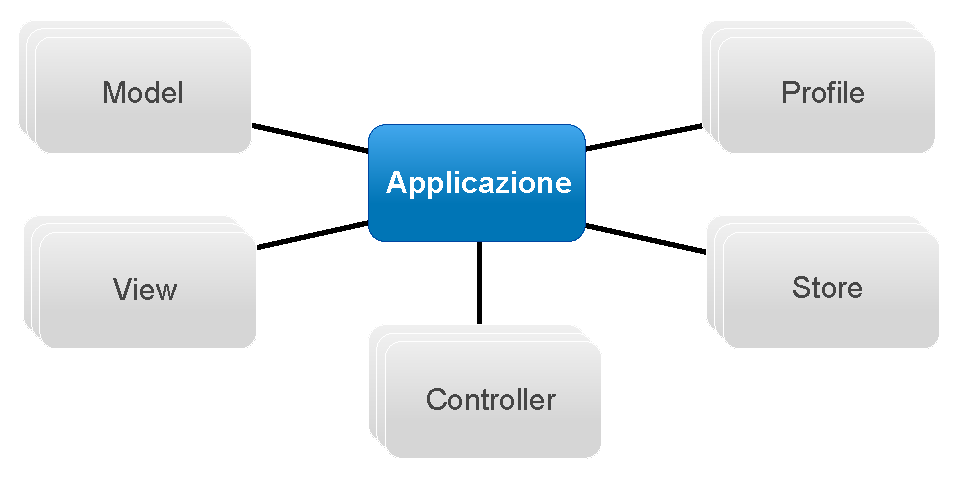
\includegraphics[keepaspectratio=true, width=\textwidth]{sencha-mvc}
				\caption{
					Un applicazione \senchat{} è composta da Models, Views,
					Controllers, Stores e Profiles
				}
				\label{fig:sencha_mvc}
			\end{figure}
			
			Come tutte le applicazioni ibride, anche quelle realizzate con
			\senchat{} hanno la possibilità di accedere a funzionalità proprie
			dei dispositivi (come utilizzare la fotocamera, ottenere la posizione
			dal GPS e avere accesso al file sys\-tem) tramite le opportune API
			della famiglia \verb|Ext.device.*|. A questo punto vale la pena
			spendere qualche parola in più per chiarire alcuni dettagli sul
			sistema di impacchettamento delle applicazioni. Per poter compilare
			l'applicazione in un pacchetto nativo installabile è necessario
			avere a disposizione gli SDK relativi alle piattaforme di destinazione.
			\senchacmd{}, una volta configurato, è in grado di creare pacchetti
			solo per piattaforme Android e iOS, ma dalla versione 2.3 è stato
			inserito il supporto per lavorare insieme a \pg{} e Cordova così da
			riuscire a supportare anche Windows Phone e BlackBerry. Un aspetto
			importante da sottolineare è che se si decide di lavorare con uno
			qualunque di questi framework, l'uso delle API \verb|Ext.device.*| per
			l'accesso al dispositivo rimane ancora valido; sarà \senchacmd{} che
			durante il processo di compilazione si occuperà di utilizzare le
			relative API Cordova o \pg{} necessarie. Un altro aspetto da
			tenere in considerazione è il fatto che se si utilizza Cordova è
			ancora necessario lavorare insieme agli SDK di Windows Phone e BlackBerry
			che devo essere presenti in locale; se invece si utilizza \pg{} è
			possibile ovviare a questo inconveniente utilizzando il suo servizio
			di compilazione online \pgb{}. Qualunque soluzione si scelga di
			adottare, dopo aver creato un progetto, è sufficiente utilizzare
			ancora \senchacmd{} per abilitare il supporto di Cordova o \pg{} e,
			fatto questo, i comandi per la compilazione rimarranno gli stessi.
			
			\senchat{}, a differenza di altri della sua categoria, non è un
			framework che offre	solo la propria shell nativa per creare
			applicazioni ibride: tra le	proprie APIs sono disponibili numerosi
			widgets per creare una consistente interfaccia grafica
			(vedi fig.~\ref{fig:senchaui}) così da non dover ricorrere a
			framework aggiuntivi come nel caso di \pg{} e \rhom{}. Sono anche
			forniti numerosi temi con aspetto nativo per le piattaforme che
			supporta, e all'interno del file di configurazione dell'applicazione
			\verb|app.json| è possibile specificare quale tema utilizzare a
			seconda della piattaforma rilevata in fase di caricamento.
			\begin{figure}[h]
				\centering
				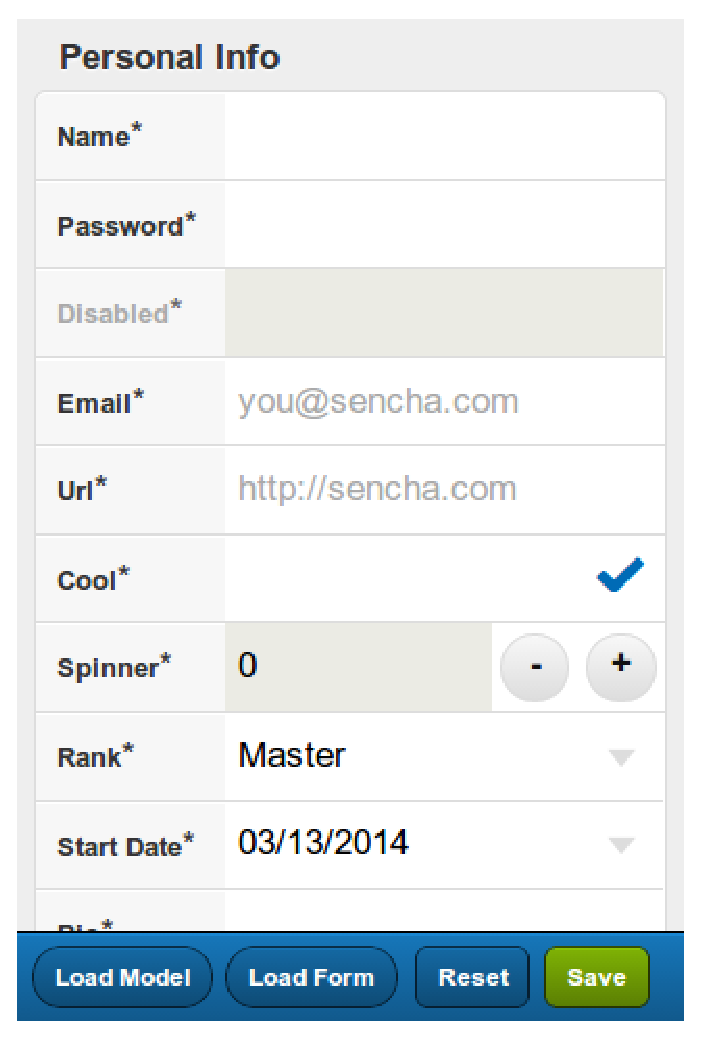
\includegraphics[keepaspectratio=true, width=0.45\textwidth]{sencha-ui-1}
				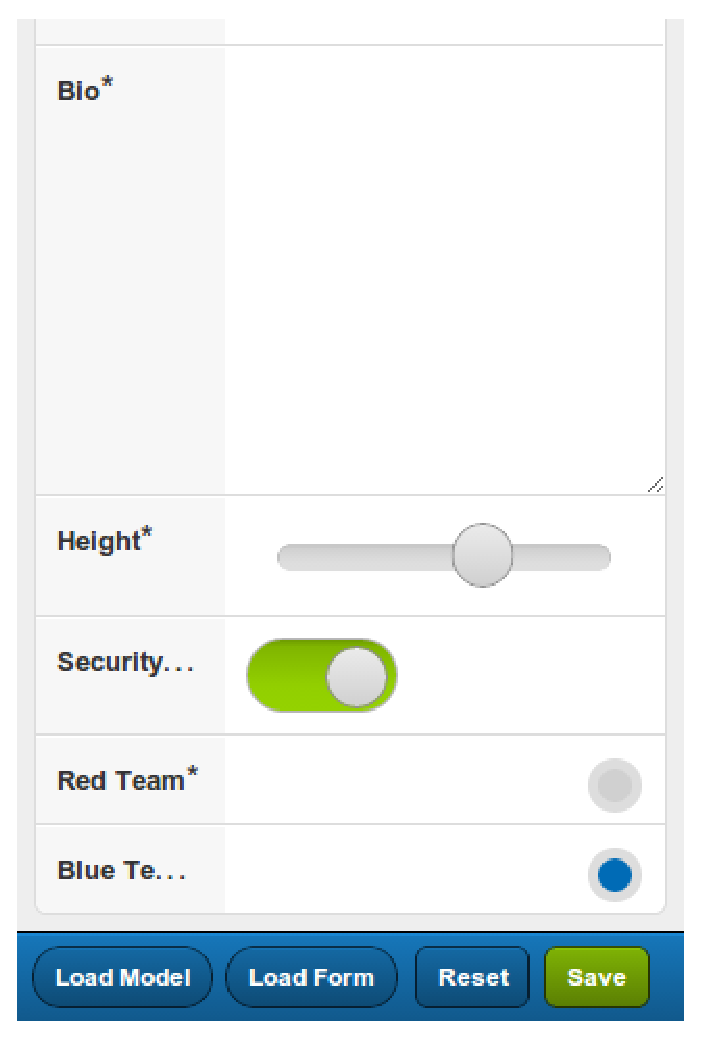
\includegraphics[keepaspectratio=true, width=0.45\textwidth]{sencha-ui-2}
				\label{fig:senchaui}
				\caption{
					Esempio di alcuni widget disponibili in \senchat{}.
					Il tema grafico mostrato è quello generico del framework e
					non specifico per nessuna piattaforma.
				}
			\end{figure}
			
	
	\section{Conclusioni}
		Per questo motivo e quello... abbiamo scelto di realizzare una app di 
		prova con Phonegap e Titanium.
